\chapter{Ergebnis}

Im Kern besteht das Programm aus 3 Algorithmen.

\section{Rand Detektion}

Das Bild wird Zeilenweise durchlaufen bis ein Pixel gefunden wurde der �ber dem Schwellwert f�r das Alpha liegt. Sobald ein entsprechender Pixel gefunden wurde wird im Uhrzeigersinn nach einem Pixel gesucht der Transparent ist dessen Rechter Nachbar im alpha �ber dem Schwellwert liegt. Sobald der Start erreicht wird, ist der Pfad vervollst�ndigt und weitere Bilder werden gesucht.

\begin{figure}
	\centering
	\includegraphics[width=0.33\textwidth]{images/RimDetection1.png}
	\caption{Rand Anfang }
	\label{fig1}
	Schwarzer Pfeil: Pixel scann\\
	Gr�ner Pfeil: Pixel �ber Schwellwert\\
	Schwarzer Wei�er Pfeil: Potenzieller Pfad\\
	Roter Pfeil: Rechts vom Potenziellen Pixel\\
	Gr�ne Felder:Potenzieller Pfad punkte\\
	Gr�nes Feld gelbe Umrandung: Nachbar scann
\end{figure}

\begin{figure}
	\centering
	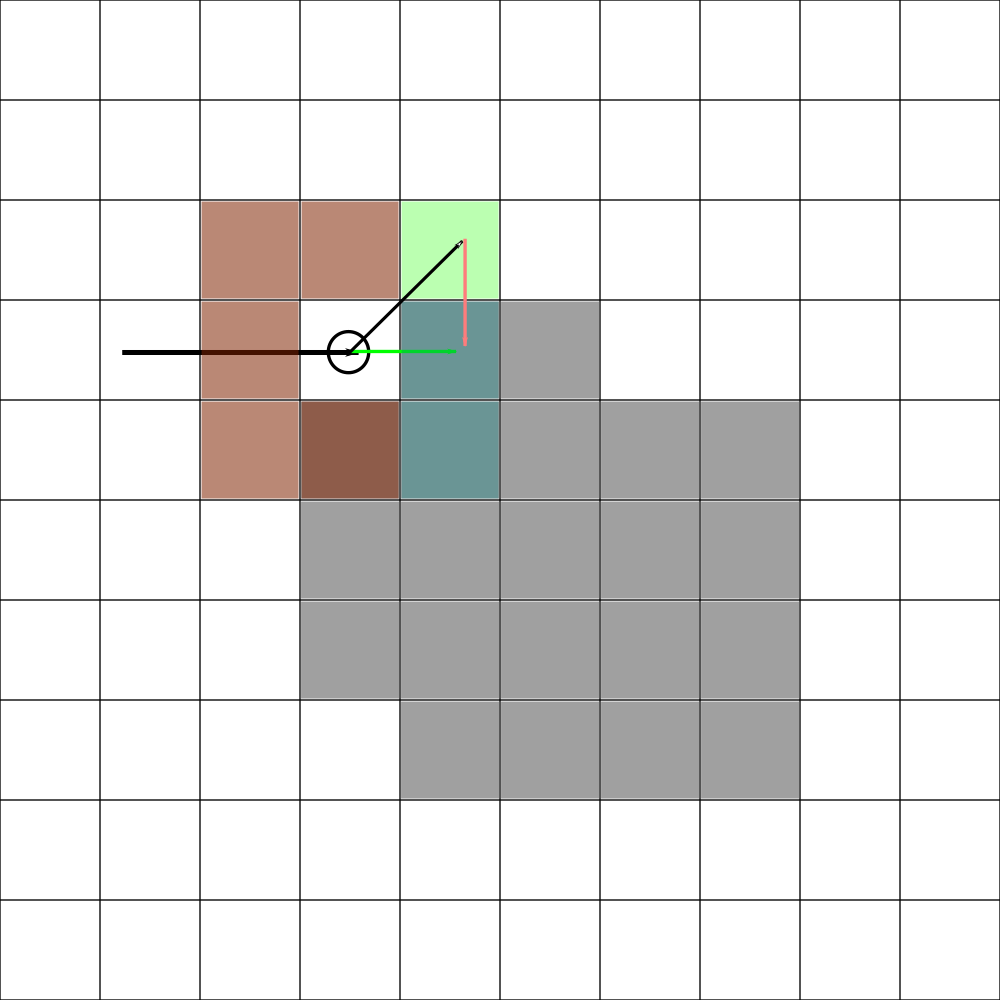
\includegraphics[width=0.33\textwidth]{images/RimDetection2.png}
	\caption{Gefundener n�chster Punkt }
	\label{fig2}
	Roter Felder:Ausgeschlossene Kandidaten \\
	Hell Gr�nes Feld: Gefundener Rand
\end{figure}

\begin{figure}
	\centering
	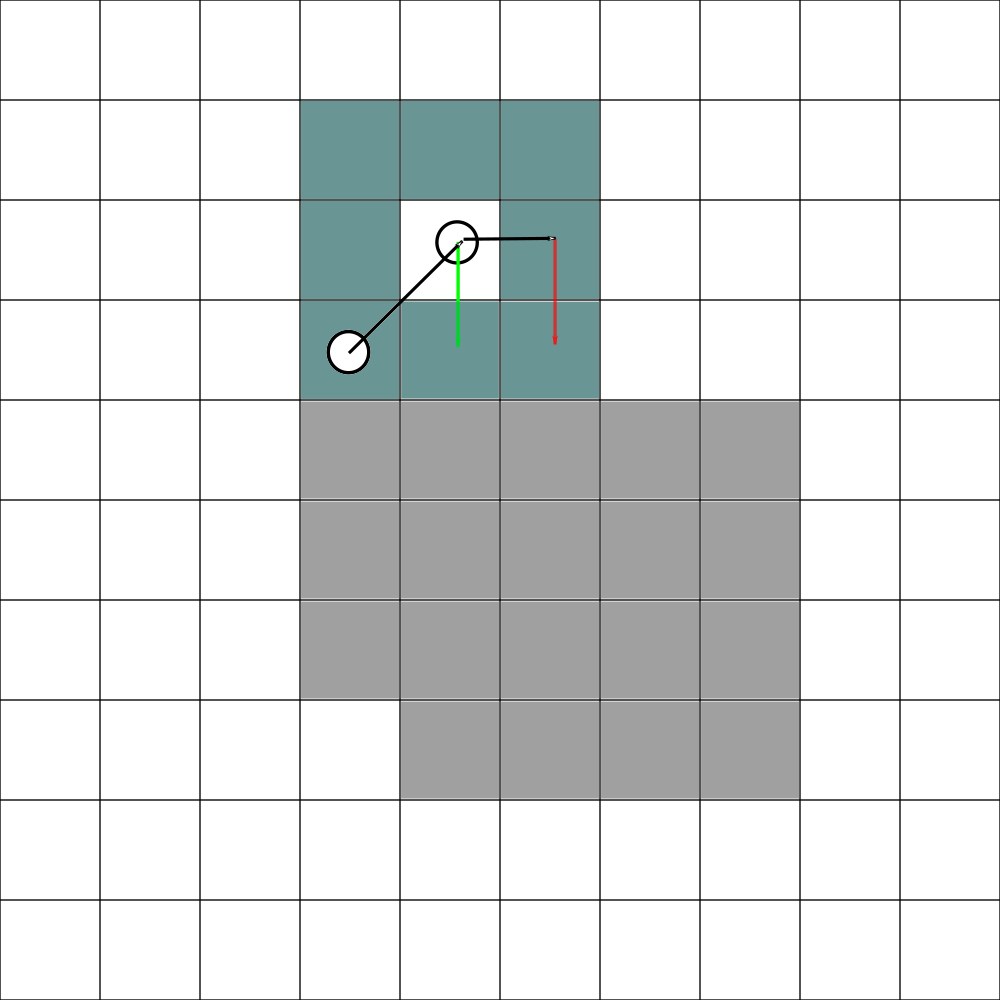
\includegraphics[width=0.33\textwidth]{images/RimDetection3.png}
	\caption{n�chster Punkt }
	\label{fig3}
\end{figure}

\begin{figure}
	\centering
	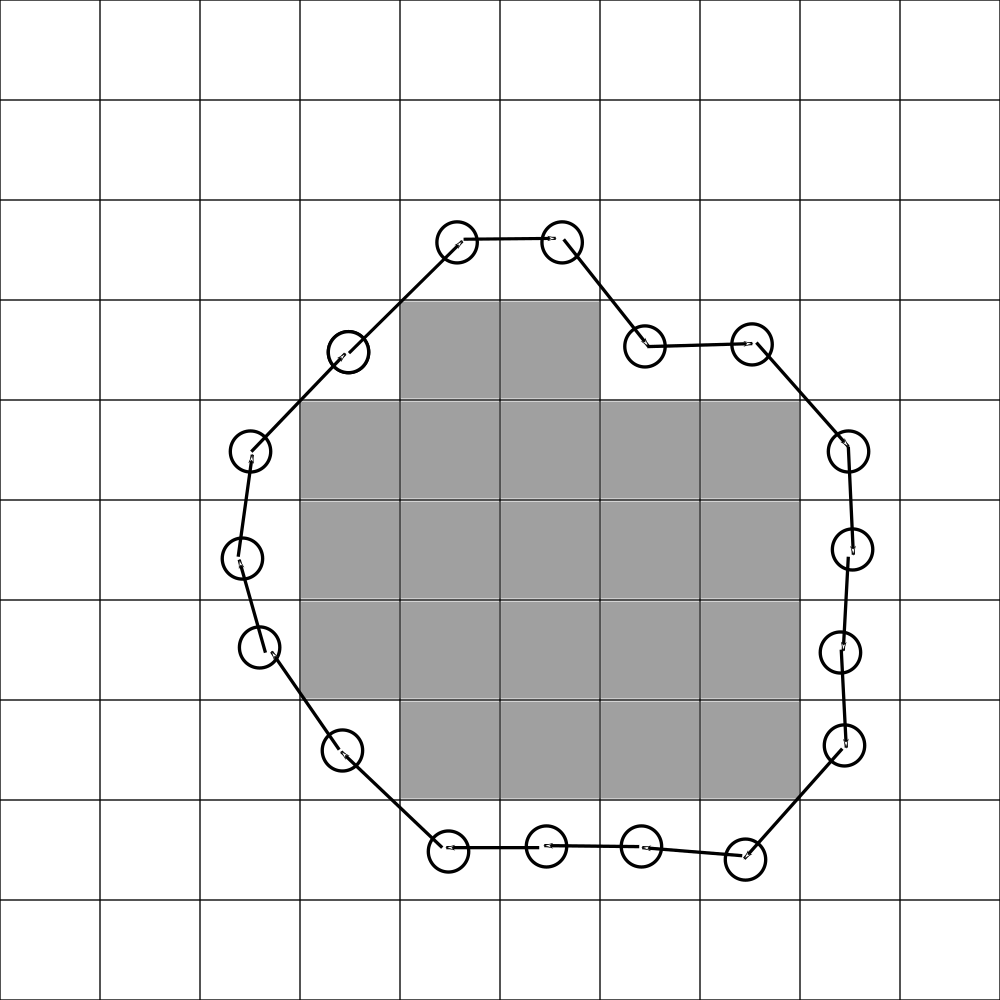
\includegraphics[width=0.33\textwidth]{images/RimDetection4.png}
	\caption{ Rand Vollst�ndig }
	\label{fig4}
\end{figure}

\section{Ramer Douglas Peucker Algorithmus}
Der Pfad besteht nun aus allen Pixeln die den Rand darstellen. Da dies auch einige Geraden beinhaltet l�sst sich der Rand gut vereinfachen um sp�ter in der Triangulierung 3-ecke zu sparen.\\
Zur Vereinfachung wird der '"Ramer Douglas Peucker Algorithmus'" verwendet. Dieser l�sst sich leicht implementieren und arbeitet zuverl�ssig.
\\
\\
Der Algorithmus sucht rekursive den entferntesten Punkt zwischen Anfang und ende. Wenn der Punkt von der Linie weiter als der Schwellwert entfernt ist wird eine Spaltung der Linie durchgef�hrt. Wenn das Maximum innerhalb des Schwellwertes ist werden Anfangs- und Endpunkt direkt mit einander verbunden. \cite{Wikipedia:15}

\begin{figure}
	\centering
	\includegraphics[width=0.33\textwidth]{images/220px-Douglas_Peucker.png}
	\caption{ Liniengl�ttung nach dem Douglas-Peucker-Algorithmus }
	\label{fig5}
\end{figure}

\section{Ear clipping}


